\chapter{Introduction}
\label{chap:introduction}

\section{Motivation}
\label{sec:motivation}
Have you ever wondered, why your images taken by your digital camera sometimes look even better than the reality? There is no magic, it starts with inevitable physics and is afterwards mainly controlled by the camera manufacturers by constructing microchips, which process the acquired images in a way such that they appear much more visually pleasing. But sometimes, this enforced beauty is also a curse.

Many computer vision algorithms rely on the assumption, that the input images have a linear relationship to the real-world scene radiance recorded at the camera sensor. For instance, on a very low level, the latter is needed for an accurate comparison of images from two different digital cameras. Another example for more complex analysis is to use the brightness values in digital images as physical measures.

One of these applications using the latter is the estimation of the illuminant color as done in \cite{tancolorconstancy}, which on the other hand has significant impact on a variety of computer vision problems like \emph{Color Constancy} \cite{finlayson2001color} or the related \emph{Color Constant Color Indexing} \cite{funt1995color} for the retrieval of images from databases. Another frequently used application is the construction of high dynamic range (HDR) images without having a special purpose camera. Techniques are proposed in \cite{mann1995being, CAVE_0068} and \cite{debevec2008recovering}. \emph{Photometric Stereo} methods \cite{woodham1980photometric, basri2007photometric} recover the shape and reflectance properties of an object using multiple images with varying lighting conditions, but a fixed viewpoint. \emph{Shape from Shading} \cite{zhang1999shape} is some kind of a special case for the latter, where the observation is just a single image. A result from such an algorithm is shown in \autoref{fig:shapefromshading}.

\begin{figure}
	\centering
	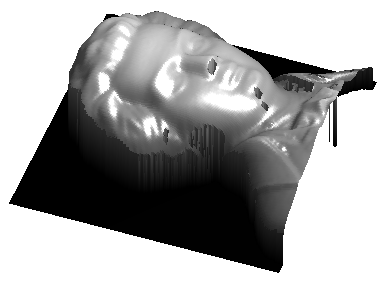
\includegraphics[width=0.3\textwidth]{images/shapefromshading.png}
	\caption[Example result of \emph{Shape from Shading}]{Example result of \emph{Shape from Shading}. Picture courtesy of R. Zhang.}
	\label{fig:shapefromshading}
\end{figure}

However, due to nonlinear camera response functions (CRF), for most digital cameras, this assumption does not hold, \hbox{i.e.} the linearity is not maintained in the observed image. Therefore, the \emph{relinearization} of the measured image intensity is very important for the above mentioned and many other algorithms to work properly. To do so, the particular CRF must be estimated and inverted. This inverted CRF can be applied to the measured image intensities to obtain an image approximately linear to the real-world scene radiance.





\section{Related Work}
\label{sec:relatedwork}
There is a huge literature on the estimation of camera response functions. Primarily it can be separated into techniques requiring special equipment, methods using several images of the same scene with known but varying camera settings and on the other hand approaches, which only need very limited information, trying to estimate the CRF from only a single intensity image. The latter are the only methods which can both operate under laboratory conditions, \hbox{i.e.} possessing the examined camera and possibly some equipment, but also when just the image and no additional knowledge is available. For instance, this is the case if the examination of camera responses from images downloaded from online resources like \emph{picasaweb} or \emph{flickr} is targeted. The two methods implemented during the creation of this thesis can both operate on single images.

The probably most popular example, where special equipment is required, is the estimation using a color chart of known reflectances like a Macbeth chart \cite{chang1996rgb}. This chart includes a set of patches in different shades of gray, starting from white and ending up in black, as well as other precisely defined colors, all in all 26 distinctive patches. These can be used to obtain some discrete samples of the actual CRF. The biggest problem here is to ensure uniform lighting.

One approach is to use a high quality light source inside a large dark room. The light source should be as far away from the chart as possible. Another approach is to place the chart outdoors under direct illumination. Note that the results will differ under these two conditions, because the illumination color will be different. 

\begin{figure}[htbp]
  \centering
  \subfigure[shortest period]{
    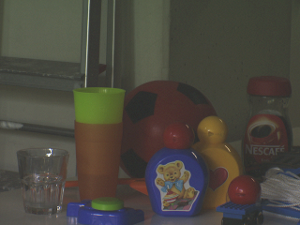
\includegraphics[width=0.22\textwidth]{images/exposure0.png} 
  }
  \subfigure[short period]{
    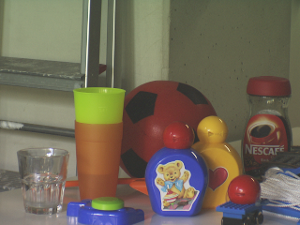
\includegraphics[width=0.22\textwidth]{images/exposure1.png} 
  }
  \subfigure[long period]{
    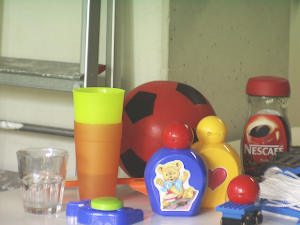
\includegraphics[width=0.22\textwidth]{images/exposure2.png} 
  }
  \subfigure[longest period]{
    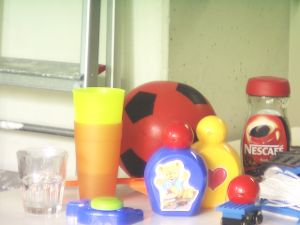
\includegraphics[width=0.22\textwidth]{images/exposure3.png} 
  }
  \caption[Estimating CRF by changing exposure settings]{Estimating CRF through changing exposure settings. Multiple same-scene images with varying exposure periods are required.}
  \label{fig:multipleexposures}
\end{figure}

Due to the fact that the camera response is a continuous function, some kind of interpolation incorporating these sampling points is applied. In theory, the effects of this interpolation have also to be inverted. Nevertheless, this manual technique provides ground-truth values. Hence, it is utilized for measuring fitting scores of different CRF approximation models, for instance the empirical model of response (EMoR) presented in \cite{CAVE_0091}, the polynomial model from \cite{CAVE_0068}, gamma curves as used in \cite{mann1995being} and \cite{farid2001aa} or the generalized gamma curve model from \cite{ng_cvpr07} presented in \autoref{subsubsec:ggcm} of this thesis.

S. K. Nayar and T. Mitsunaga presented the ``Radiometric Self Calibration'' in 1999 \cite{CAVE_0068}. This algorithm requires a set of images of an arbitrary scene, captured with several different exposure settings (for an illustration see \autoref{fig:multipleexposures}). For each image, different shutter speed configurations and different aperture settings are used. The primarily intended application for this method is the automatic generation of accurate high dynamic range images. A demonstration is available on their website\footnote{\url{http://www.cs.columbia.edu/CAVE/software/rascal/rrhome.php}}.

Another CRF estimation approach introduced by the same authors was published one year later, titled ``High Dynamic Range Imaging: Spatially Varying Pixel Exposures'' \cite{nayar2000high}. Here, they utilize an optical filter with spatially varying transmittance and they show that this variation has a certain correspondence to the irradiance ratio. This information is used to estimate the CRF from a single image and thus their approach -- unlike the one published one year earlier -- does not require to capture a whole set of images of a static scene using separate camera settings.

A more recent method published in 2008 \cite{takamatsu2008estimatingECCV} requires several static same-scene images, but without varying the camera settings. J. Takamatsu, Y. Matsushita and K. Ikeuchi use a so-called \emph{Probabilistic Intensity Similarity Measure} (PISM), which represents the likelihood of two intensity observations corresponding to the same scene radiance. Due to the presence of noise, having two or more images of the same scene, these observations will slightly differ. They show that the PSIM is strongly related to the particular CRF and thus maximizing this intensity similarity function for all pixels over a set of same-scene images leads to a reliable estimation of the camera response. Unlike other methods, this one is independent of any particular statistical prior models. Real-world experiments demonstrate the effectiveness of this method for digital cameras as well as video cameras.

In ``Blind Inverse Gamma Correction'' \cite{farid2001aa}, H. Farid measures the effects of the gamma correction from a single image without any knowledge of the used camera or any calibration information. It is shown on both, natural and synthetic images, that the error between the estimated and the ground-truth gamma curve is in most cases very small. But the problem here is, that for almost every real-world camera, the camera response is a combined effect of various internal operations, not only gamma correction. Hence, this method does not really fit to the approach of estimating a complete CRF.





\section{Patents}
\label{sec:patents}
There are two relevant patents related to publications by S. Lin et \hbox{al.} US patent 7450754 from November 2008 is entirely based on \cite{Lin04radiometriccalibration} and thus the claimed method requires three channel RGB images for estimating the CRF. Due to this method being part of this thesis, it is described in detail in \autoref{sec:radcal}. The application number is 10/809167, filed in March 2004. The 2005 filed (application number 11/156988) US patent 7463769 issued in December 2008 claims another approach, ``Determining the Radiometric Response Function from a Single Grayscale Image'' \cite{lin2005determining}, which uses a statistical feature of graylevel histograms at edge regions to gain information for radiometric calibration. This method is -- as its name implies -- intended for grayscale images, but can also be used for images with more than one channel by analyzing each channel separately. The approach can be seen as a grayscale pendant to \cite{Lin04radiometriccalibration}. Hence for both, color and grayscale images, their methods are covered by US patents.

Another related US patent numbered 7505606 from March 2009, filed on May 2005, is titled ``Detecting Doctored Images using Camera Response Normality and Consistency'', where parts of the method proposed in the identically named publication \cite{rongrong-detecting} are claimed. Sets of patches of an image containing cues on the applied CRF are obtained. A support vector machine (SVM) is trained with some features extracted from examples of normal and abnormal inverse CRFs to be able to classify given inverse CRFs into normal and abnormal ones. This method helps distinguishing natural and tampered images. Although the recovery of inverse CRFs from images to map the intensities back to irradiance is mentioned in their list of claims, it is not presented in detail. Some figures shown in the drawings part are very similar to those in a publication of an approach presented in this thesis \cite{Lin04radiometriccalibration}, but the claims are mainly on training the SVM and classifying sets of patches for image forensics. So this patent does not severely limit implementations of CRF estimation.

All three patents above are assigned to \emph{Microsoft Corporation}, Redmond, WA (US).



\section{Thesis Overview}
\label{sec:overview}
In \autoref{chap:crf}, an overview of the camera-internal processes is given. The first step, the measuring of scene radiance is presented in \autoref{sec:radiancetoirradiance} and the second step, the transformation from image irradiance to image intensity in \autoref{sec:irradiancetointensity}. Afterwards, in \autoref{chap:description} the two methods treated in this work are described, starting with \cite{Lin04radiometriccalibration} in \autoref{sec:radcal}. The second method \cite{ng_cvpr07} is described in \autoref{sec:geoinv}. In \autoref{chap:evaluation}, at first, a short overview of the problems we encountered when implementing the second method is given in \autoref{sec:challenges}. The actual evaluation is about the first approach and starts with the examination of the capabilities of the data acquisition step in \autoref{sec:capabilitiesofdataacqu} by varying two crucial parameters. Tests with synthetic data in \autoref{sec:syntheticdata} demonstrate the influence of the parameter $\lambda$. In \autoref{sec:stability} the robustness of the method is examined by utilizing sets of same-camera images. Finally, in \autoref{chap:summaryoutlook}, a short summary and outlook are given.